\section{State Space Analysis}
\label{sec:State_Space_Analysis}

\subsection{Sample Deployment}

We briefly illustrate the timing analysis methods and lessons learned using a simple example. This is a 3-satellite cluster (Figure \ref{fig:CT}) with each satellite running instances of a mixed-criticality DREMS application. Each satellite consists of a set of sensor-dependent critical components required for both safe flight and remote sensing tasks. These components interact with physical sensor devices such as cameras, GPS receivers, etc. periodically invoking functions, processing data and communicating with a ground station. 

\vspace{-0.1in}
\begin{figure}[htb]
	\centering
	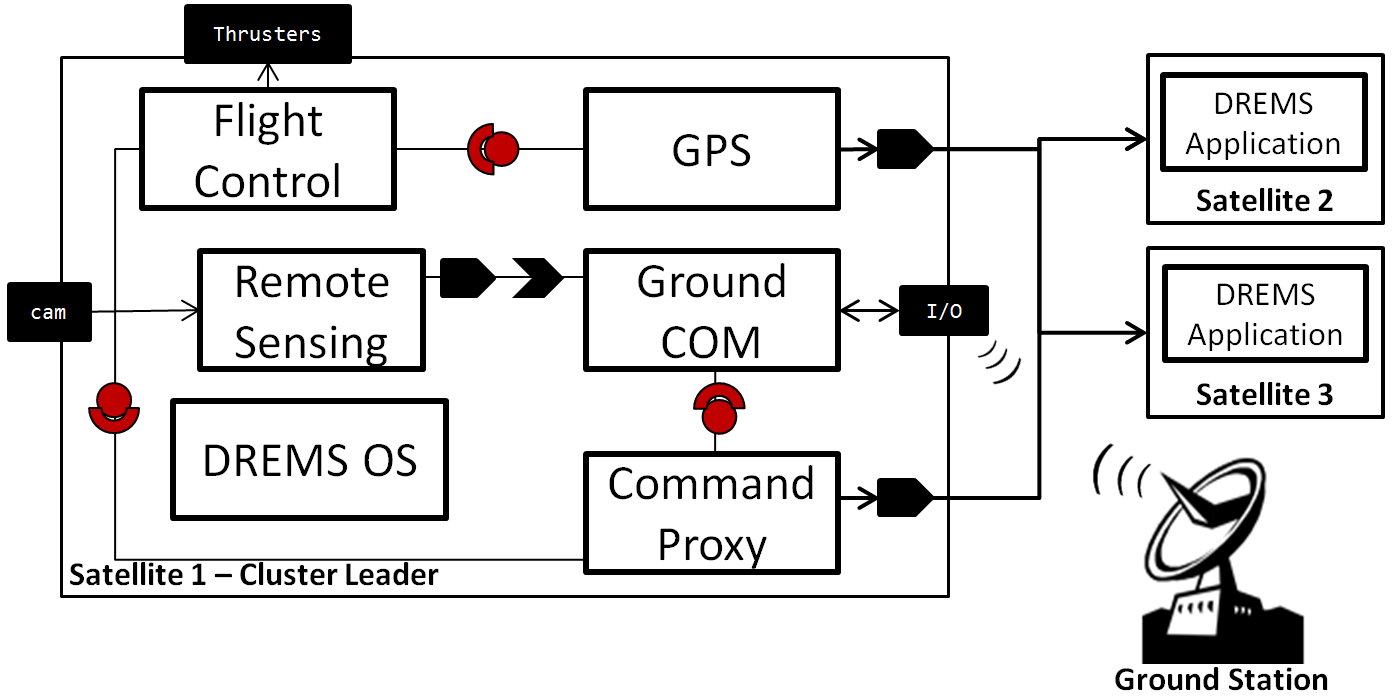
\includegraphics[width=0.40\textwidth]{figs/Case_Study_Fixed.png}
	\caption{A DREMS Application}
	\label{fig:CT}
\end{figure}

A \emph{GPS} component periodically publishes a state vector to all satellites in the cluster. The \emph{Flight Control} component uses an RMI interface to access the most recent state vector from the GPS including data received from other satellites to calculate and maintain the flight trajectory. %The Flight Control component does not fetch GPS information until all the satellites have published on the updated sensor data. 
There are situations when the ground station will command the satellites in the cluster to perform a coordinated \emph{scatter} maneuver; this is a time-critical event that is initiated by a transmission to the cluster leader satellite. On receiving such a command, the \emph{Ground COM} of Satellite 1 uses an interface on the \emph{Command Proxy} to publish this command to all satellites in the cluster. This proxy uses a high-priority synchronous RMI to communicate with the Flight Control component to trigger the scatter. Since the component-level scheduler is non-preemptive, the Flight Control cannot suspend any operation that it could be executing at time $t_S$ when a scatter request is received from the Command Proxy. %This motivates the need for accurate modeling of component interaction semantics to obtain conservative response-time results. 
The abstract business logic \emph{steps} of the \emph{scatter} operation in the Flight Control is modeled as shown in Figure \ref{fig:FLC}.

%This operation is requested by the Command Proxy when a command is received from the ground station. For sake of simplicity, we have reduced this operation down to 3 distinct steps. The controller first obtains updated position vectors from the GPS component using the RMI interface. \iffalse Notice the lack of a WCET for this interaction. This is because the GPS is scheduled on a separate temporal partition and the amount of time for which the Flight Control has to wait for the updated metrics is dependent on the time stamp at which the scatter command is received and also the state of the GPS component message queue.\fi Once these metrics are received, the Flight Control calculates a new trajectory. Once the trajectory is calculated, each Flight Control component interacts with the thrusters and maneuvers the satellites.  

\vspace{-0.1in}
\begin{figure}[htb]
	\centering
	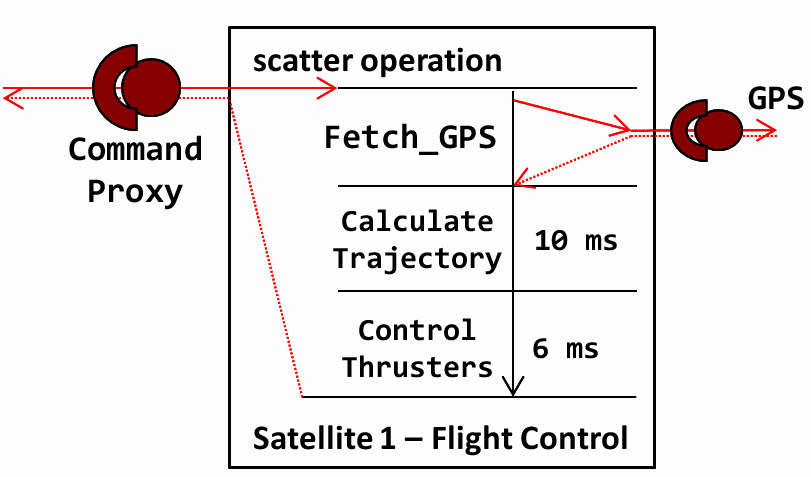
\includegraphics[width=0.30\textwidth]{figs/scatter.jpg}
	\caption{Steps of the Scatter Operation}
	\label{fig:FLC}
\end{figure}

%\vspace{-0.1in}

The temporal partition schedule for this scenario consists of two minor frames of length 100 msec each. All satellite sensor components such as the camera and the \emph{GPS} are grouped into sensor processes and assigned to the first temporal partition. The \emph{Flight Control} is assigned to partition 2 and is guaranteed to receive the newest vector data as it waits for the \emph{GPS} component to update the database of state variables. The \emph{Ground COM} and the \emph{Command Proxy} component threads run at high priority and are scheduled on demand. 

Although in a realistic deployment the network performance is dependent on the satellite's momentary position, we have assumed worst-case network delays on all data links. This is a simplification on the amount of information the CPN model needs to hold that can tightened by a more detailed, time-dependent model. 
% This abstraction can be tightened by integrating the network profile of each port into the design model. This profile will take the form of a list of records, each record being the tuple $<t_i, Bandwidth_{t_{i}}>$, $0 \le t_i \le P_{o}$, where $P_{o}$ is the orbital period. 

%\vspace{-0.1in}

%\iffalse
\begin{table*}[t]
  \small
	\caption{Component Operations on Satellite 1}
	\label{table:AR}
	\begin{center}
		\begin{tabular}{ | c | p{2.0cm} | p{1.7cm} | p{1.7cm} | p{1.7cm} | p{1.9cm} | p{1.9cm} |}
			\hline
			Component & \multicolumn{1}{|c|}{Operation} & $Dl_{O}$ (ms) & $T_{NQ}$ (ms) & $T_{DQ}$ (ms) & $T_{FIN}$ (ms) & $T_{EXEC}$ (ms) \\ \hline
			GPS & \multicolumn{1}{|c|}{publish\_vector} & \multicolumn{1}{|c|}{10} & \multicolumn{1}{|c|}{0} & \multicolumn{1}{|c|}{0} & \multicolumn{1}{|c|}{8} & \multicolumn{1}{|c|}{8} \\ \hline
			GPS & \multicolumn{1}{|c|}{update\_dbs} & \multicolumn{1}{|c|}{18} & \multicolumn{1}{|c|}{20 (n/w delay)} & \multicolumn{1}{|c|}{20} & \multicolumn{1}{|c|}{36} & \multicolumn{1}{|c|}{16} \\ \hline
			Remote Sensing & \multicolumn{1}{|c|}{img\_process} & \multicolumn{1}{|c|}{90} & \multicolumn{1}{|c|}{0} & \multicolumn{1}{|c|}{12} & \multicolumn{1}{|c|}{80} & \multicolumn{1}{|c|}{80} \\ \hline
			Ground COM & \multicolumn{1}{|c|}{transmit\_imgs} & \multicolumn{1}{|c|}{20} & \multicolumn{1}{|c|}{80} & \multicolumn{1}{|c|}{80} & \multicolumn{1}{|c|}{95} & \multicolumn{1}{|c|}{15} \\ \hline
			Ground COM & \multicolumn{1}{|c|}{scatter\_cmd} & \multicolumn{1}{|c|}{200} & \multicolumn{1}{|c|}{120} & \multicolumn{1}{|c|}{120} & \multicolumn{1}{|c|}{315} & \multicolumn{1}{|c|}{195} \\ \hline
			Command Proxy & \multicolumn{1}{|c|}{notify\_cmd} & \multicolumn{1}{|c|}{200} & \multicolumn{1}{|c|}{132} & \multicolumn{1}{|c|}{132} & \multicolumn{1}{|c|}{142} & \multicolumn{1}{|c|}{10} \\ \hline
			Flight Control & \multicolumn{1}{|c|}{calc\_trj} & \multicolumn{1}{|c|}{45} & \multicolumn{1}{|c|}{100} & \multicolumn{1}{|c|}{100} & \multicolumn{1}{|c|}{150} & \multicolumn{1}{|c|}{50} \\ \hline
			Flight Control & \multicolumn{1}{|c|}{scatter} & \multicolumn{1}{|c|}{200} & \multicolumn{1}{|c|}{142} & \multicolumn{1}{|c|}{150} & \multicolumn{1}{|c|}{305} & \multicolumn{1}{|c|}{163} \\ \hline
			
			
		\end{tabular}
	\end{center}
	\vspace{-0.2in}
\end{table*}
%\fi

\subsection{State Space Exploration}


The CPN Tools uses a built-in state space (SS) analysis tool to generate a bounded state space from an initial CPN model. However, it has been previously noted \cite{CPNTwoInterfaces} that the built-in state space tool is inefficient with its search algorithm. We therefore also use the ASAP tool \cite{ASAP} to utilize advanced analysis methods \cite{Christensen2001}. For smaller design models such as the above deployment, we also use observer places \cite{Alpern1989} in the CPN to \emph{collect} tokens that represent timing anomalies such as deadline violations.

Components in safety-critical DRE applications can be either sporadically or periodically triggered. A bounded state space generated in CPN Tools must be sufficiently complete so that the lack of deadline violations, deadlocks, or delayed responses \emph{within} a chosen execution interval will guarantee safe operation throughout the complete lifetime of the applications. Table \ref{table:AR} shows some worst-case execution time results from state space analysis on each component thread on Satellite 1. Each operation request is enqueued into the component message queue at time $T_{NQ}$. A dispatcher thread dequeues this request at $T_{DQ}$ and schedules an operation for execution. Once scheduled, the component executor thread executes each operation to completion at time $T_{FIN}$ leading to an overall execution time of $T_{EXEC}$ measured from $T_{NQ}$. These results allow the verification of several timing properties. 

\textbf{Lack of System-wide Deadlocks:} System-wide deadlocks are caused by the inability of the OS schedulers (on any of the nodes) to schedule any component thread, e.g., due to infinite thread blocking. Deadlocks are identified by checking the firing conditions on leaf node transitions in the state space tree. Deadlock faults are also isolated by detecting operation timing violations, prolonged thread blocking (as observed in the place \emph{Blocked Threads}) and idle scheduler behavior. 

\textbf{Lack Deadline Violations:}
%On a sufficiently large bounded state space, the analysis tool looks for specific behavioral patterns such as weakly-decreasing size of the component message queue.
%A \emph{Deadline\_Violation} (Figure \ref{fig:DL}) transition fires at any point in time when the guard \emph{dl\_guard} is satisfied and arc bindings are realized with its input places.
A deadline violation is observed when a component operation takes longer to complete than its set \emph{deadline}. The deadline is computed starting from the time when the operation is marked as \emph{ready}. For every operation $O$ that is either waiting in the message queue or currently executing, a violation \emph{DLV(O)} is detected in accordance with Equation \ref{eq:DLV}.

\vspace{-0.1in}
\begin{equation}
\label{eq:DLV}
DLV(O)= 
\begin{cases}
true,& \text{if } T_{NC} - T_{NQ_{O}} > T_{DL_{O}}\\
false,              & \text{otherwise}
\end{cases}
\end{equation}

where $T_{NC}$ is the current node clock value and $T_{NQ_{O}}$ is the time value at which the operation is enqueued onto the component message queue. If the elapsed time is longer than the operation's deadline $T_{Dl_{O}}$, a violation flag is set. At each state space node, the \emph{SearchNodes} function of CPN Tools is used with the \emph{DLV(O)} predicate to identify violated deadlines. However, the \emph{search area} for this function must be carefully chosen. If the search area is small, the analysis may become shortsighted and incorrect. If the search area is too large (the entire tree), the query would take a long time to execute. For our simple example we generated a state space of upto 200,000 nodes covering a sufficiently large 10 hyperperiods of thread activity and varying thread priorities on all hardware nodes.

\textbf{Worst-case Response time Analysis:}
Although a complete lack of deadline violations on the operation-level is important for timeliness of a component, it is often the case in distributed systems that a developer is more interested in end-to-end latencies between specific events. The response time for a system-level service may be dependent on timely execution of several \emph{interacting} component operations. Specifying upper bounds for response times is also easier for a system integrator compared to providing deadlines for each operation. Here lies an analytical trade-off where a bounded trigger-to-response time would be sufficient even if one or more operations that enable the response violate individual deadlines. 

The worst-case response time is computed as the difference between the earliest completion time of a triggering operation and the latest completion time of a  response  operation. Each of these values is derived from a bounded state space search query that identifies all \emph{completed operations} and orders the resultant list based on $T_{FIN}$. For e.g. Table \ref{table:AR} shows a worst-case response time of 195 ms for the scatter command, observed when \emph{GroundCOM} receives a return value from \emph{scatter\_cmd}. This response requires the timely execution of \emph{notify\_cmd}, \emph{calc\_trj} and \emph{scatter} as also shown in Figure \ref{fig:FLC}. 

%\subsubsection{Search Results}

%Table \ref{table:AR} shows some worst-case execution time results from state space analysis on each component thread on Satellite 1. Each operation request is enqueued into the component message queue at $T_{NQ}$. A dispatcher thread dequeues this request at $T_{DQ}$ and schedules an operation for execution. Delays in the dequeue can be caused due to the non-preemptive nature of the component-level scheduling. Once scheduled, the component executor thread sequentially executes the steps in each operation to completion at time stamp $T_{FIN}$ leading to an overall execution time of $T_{EXEC}$ measured starting from $T_{NQ}$. 

%Significant worst-case network delays are assumed between interacting components that are distributed. For instance, the GPS component on each node finishes publishing sensor data at time stamp 8 ms but the GPS components on other nodes do not notice the subscription token in the message queues till $T_{NQ} = 20 ms$. Also, the synchronous dependency of the Flight Control component with the GPS component is a sign of poor design as a scatter command received in partition 2 of one hyperperiod will most likely finish only a hyperperiod later as the updated GPS coordinates are queried. 

\subsubsection{Incomplete Designs}

Initial designs of real-time systems are often specified by timing requirements between system entities. For scenarios where the developers are aware of minimum timing requirements but not thread execution orders or OS-level priorities, we have applied this approach to identify partial thread execution orders to refine incomplete designs. The results of this analysis help with identifying component threads that need to be separated by temporal partitions or thread priorities in order to satisfy timing guarantees.  However, since all combinations of thread execution orders need to be observed to identify a useful \emph{execution trace}, this particular analysis does not scale well for larger component-based applications where no priority assignment has previously been made. 

%Consider a sample application that consists of 6 components servicing operation requests. Components threads 1, 2, and 3 are assigned to Partition 1 and threads 4, 5, and 6 are assigned to Partition 2. The thread priorities and execution orders are unknown. Each component is triggered by a timer once every major frame, taking up to 8 ms to complete the triggered operation. Assuming a designer requires that operation 3 (handled by thread 3) must complete before 20 ms and operation 5 (handled by thread 5) must complete before 60 ms from the start of the schedule, the analysis will provide a partial thread execution order that satisfies these requirements. To facilitate this, we assign all the relevant threads equal priorities. If all the triggering timers expire at the beginning of the partition schedule, then all component threads become eligible for execution and the OS scheduler uses a non-deterministic round-robin scheduling scheme. By querying the bounded state space that encapsulates this behavior, we arrive at a partial thread scheduling order that satisfies our requirements e.g. thread 3 is scheduled first in partition 1 and thread 5 is scheduled first in partition 2.

\subsection{Discussion}

\subsubsection{Conservative Results}

Using estimates of worst-case execution time for component operations is motivated by the need to make exaggerated assumptions about the system behavior. Pessimistic estimates are a necessary requirement when verifying safety-critical DRE systems. Schedulability analysis with such assumptions should  provide strictly conservative results. This means that (1) if the analysis results show the possibility of a deadline violation but the deployed system does not, the obtained result is a conservative one as it assumes worst-case behavior, and (2) if the analysis results do not show any timing violations but the deployed system violates response time requirements, deadlines etc., then the analysis does not provide a conservative result and has failed to verify system behavior.

In order to guarantee conservative results, the analysis must include worst-case behaviors of all system-level threads that run at higher priority than component threads and are not necessarily modeled by the design-time tools. In our analysis, these threads are grouped into a set of critical processes with approximations made to simulate the behavior of system-level threads such as (1) globally periodic CPU utilization, (2) CPU utilization for some WCET per partition. The best approximation is chosen based on the expected behavior of such critical processes. Best-effort processes are ignored as they always run at a priority lower than the lowest-priority component thread. 

\subsubsection{Scalability}
In previous efforts \cite{MoDeVVa}, we presented results showing our analysis model that it scales well for medium-sized applications, tested up to 100 mixed-criticality components distributed on up to 5 computing nodes. As the determinism in the initial design increases, the number of possible behaviors and therefore the size of the state space decreases. In essence, the effort required for the analysis to be useful to the designer is dependent heavily on the initial design itself. Increasing the number of equally prioritized components will exponentially increase thread scheduling opportunities and the size of the state space required to accumulate the tree of component behaviors.  %Although these results were based on design models that made some unrealistic assumptions e.g. 100 timers expiring at the same time and triggering interactions, we have used some heuristics to reduce the generated state space and improve the performance of the search methods. 


%\paragraph{Symmetry}
%One of the main advantages of using component-based design for complex systems is reusability. It is not unusual to deploy instances of the same application with the same component assembly on multiple hardware nodes. If these applications are deployed on symmetrical nodes, the observed state space of behaviors will also be symmetrical. To enable efficient search through symmetrical state spaces, we use symmetry-based state space reduction techniques \cite{Kristensen2000} to improve the performance. This is handled by 

%In Figure \ref{fig:hl_cpn}, to model 100 timers, we moved from using 100 colored tokens in the \emph{Timers} place to using a single token which is a list consisting of a 100 elements. This way, when multiple timers expire, a single transition firing handles all the expiries across all nodes (a single state change) instead of multiple transition firings leading to multiple new states. However, the non-determinism caused by the OS-level scheduling will still affect the state space even across symmetric deployments.  
%\paragraph{ASAP Tool}
%The ASAP tool provides for several search algorithms and state space reduction techniques such as the \emph{sweep-line method} \cite{Christensen2001} which deletes already visited state space nodes from memory, forcing on-the-fly verification of temporal properties. One of the disadvantages of using such heuristics is the run-time cost incurred by backward-generation of states when a backtrace for a violation is required. However, if a path from the initial state to an inconsistent state is not desired, a combination of this method and the symmetry method reduces the state space and improves verification performance.  

\section{Integration of Modeling Tools}
\label{sec:IMT}

This section briefly describes the integration of the CPN-based analysis with the design-time modeling tools for automated model transformations and code generation. By parsing the domain-specific model of the system, obtaining the necessary structural and behavioral attributes and using a model interpreter, a valid CPN model for the design is automatically generated.

\subsection{Timing Specification for Component Operations}

As mentioned in Section \ref{para:steps}, every component operation is modeled as a sequence of functional steps, each with an assigned worst-case execution time. Our goal with this specification is to be able to model these sequential steps. We broadly classified these steps into (1) local code blocks, (2) peer-to-peer synchronous and asynchronous remote calls, (3) anonymous publish/subscribe distribution service calls, (4) blocking  and non-blocking I/O interactions, and (5) bounded loops. The restriction to these 5 types is a consequence of the DREMS component model and can be easily expanded. 

Figure \ref{fig:ANTLR} shows an example temporal specification for the operation \emph{on\_one\_data} residing in Component \emph{Trajectory\_Planner} exposed through the \emph{Sensor\_Data\_Subscriber} port. This port subscribes to sensor data published by another component using \emph{Push Subscription} semantics. On reception of sensor data, the operation \emph{on\_one\_data} is called, triggering a sequence of events. Abstracting the business logic, this operation has 4 execution steps: (1) local \emph{work} for 12 ms, followed by an (2) RMI call to the remote method \emph{fetch\_data} using the \emph{Fetch\_Sensor\_Data} receptacle port, (3) 16 ms of local work, and finally (4) publishing a \emph{Plan} data structure anonymously using the \emph{Notification\_Publisher} port. 

\vspace{-0.1in}
\begin{figure}[htb]
	\centering
	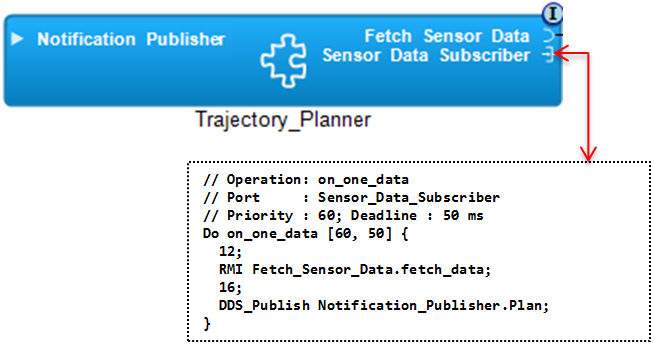
\includegraphics[width=0.50\textwidth]{figs/Timing_Specification.png}
	\caption{Timing Specification for Component Operation}
	\label{fig:ANTLR}
\end{figure}

\vspace{-0.1in}  

\subsection{Model Generation}

A model interpreter parses the design model tree and builds data structures representing the various CPN tokens described in Section \ref{sec:Colored_Petri Net-based_Analysis_Model}. This includes structural properties like component assembly and software deployment, temporal properties like scheduling schemes, operation execution times and instantiated deployment where a single application can be deployed simultaneously on multiple computing nodes. %Figure \ref{fig:GT} shows the token structure generated for the on\_one\_data operation.
Using text templates, a modular and hierarchical CPN model is generated.

\iffalse
\begin{figure}[htb]
	\centering
	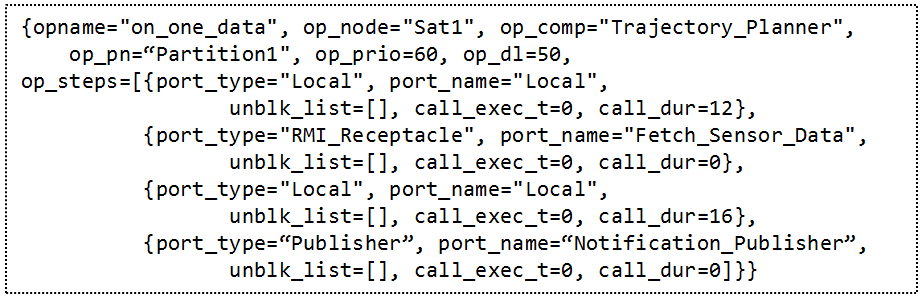
\includegraphics[width=0.48\textwidth]{figs/Generated_Token.png}
	\caption{on\_one\_data CPN token}
	\label{fig:GT}
\end{figure}
\fi 


